\documentclass[review]{elsarticle}

\usepackage{lineno,hyperref}
\modulolinenumbers[5]

\journal{Expert Systems with Applications}

\usepackage[figuresright]{rotating}
\usepackage{graphicx}
\usepackage{subfigure}
\usepackage{times,amsmath,epsfig}
\usepackage{amssymb}
\usepackage{slashbox}
\usepackage{multirow,multicol}
\let\algorithm\relax
\let\endalgorithm\relax
\usepackage[linesnumbered,ruled,boxed,vlined]{algorithm2e}

\usepackage{color}

\newtheorem{definition}{Definition}
\newtheorem{lemma}{Lemma}
\newtheorem{corollary}{Corollary}
\newtheorem{proof}{Proof}

\newcommand{\modify}[1]{\textcolor{blue}{#1}}
\newcommand{\fixme}[1]{\footnote{\textcolor{red}{\textbf{FIXME!!!} #1}}}
%\let\modify\     %% remove the left %, if we want to change red to black


\begin{document}

\begin{frontmatter}

\title{Refreshment of the Shortest Path Cache with Change of Single Edge}

\author[address1]{Xiaohua Li}
\ead{lixiaohua@ise.neu.edu.cn}
\author[address1]{Tao Qiu}
\ead{qiutaoneu@gmail.com}
\author[address2]{Ning Wang\corref{cor}}
\ead{ningwang@shu.edu.cn}
\author[address1]{Xiaochun Yang}
\ead{yangxiaochun@ise.neu.edu.cn}
\author[address1]{Bin Wang}
\ead{wangbin@ise.neu.edu.cn}
\author[address1]{Ge Yu}
\ead{yuge@ise.neu.edu.cn}
\cortext[cor]{Corresponding author.}
\address[address1]{School of Computer Science and Engineering, Northeastern University, Liaoning, China}

\address[address2]{Department of Information Management, School of Management, Shanghai University, Shanghai, China}

%% \address[mymainaddress]{College of Information Science and Engineering,\\
%% Northeastern University, Liaoning 110819, China\\}
%% \address[mysecondaryaddress]{360 Park Avenue South, New York}

\bibliographystyle{model5-names}\biboptions{authoryear}


\begin{abstract}
The problem of caching shortest paths has been widely studied.
All existing methods that address this problem assume that the conditions of road networks do not change with time.
In this paper, we study how to refresh a cache when one edge of the underlying road network (graph) changes. A bitmap-based cache structure is proposed to store and give access to shortest paths. In the following, algorithms are developed to detect shortest paths that are affected by the change of edge. After detecting affected paths, several heuristic-based refreshment strategies are proposed to update the cache. We have conducted a series of experiments to compare the performance of proposed methods. It shows that replacing affected shortest paths with new ones whose benefit values are largest should be applied in the shortest paths caching applications such as navigation and map services.
\end{abstract}

\begin{keyword}
\texttt{shortest path caching, cache refreshment strategy, change of road network, affected shortest paths}
\end{keyword}

\end{frontmatter}

\linenumbers

\section{Introduction}
Shortest path query systems are now widely seen in our daily life \citep{wu2012shortest,potamias2009fast,wei2010tedi,liu2011generalization,
cheng2012efficient}.
People use map service for shortest paths to restaurants, parking lots, cinemas, playgrounds, shopping malls and so on.
With the uberisation, drivers of private cars also frequently use map service for various destinations.
When a user has a shortest path query, a cache in a local server is accessed; the result, if existing, will be directly returned to the user. If the cache does not have an off-the-shelf result to the query, the system accesses a global server which runs a shortest path algorithm for the query. The latter situation undoubtedly costs communication and computational time \citep{altingovde2009cost,baeza2007impact,Kriegel2008Hierarchical,gan2009improved,markatos2001caching}. The cached contents are, therefore, very critical for the efficiency of the whole caching system.

In the shortest path caching problem, all of existing works discuss the cache initialization problem which addresses how to load an empty cache when a road network and a query log are known, so that the cache works in a high level of efficiency in the future. Researchers usually load paths with the highest query frequencies into the cache, or those paths that contain the most numbers of nodes~\citep{thomsen2012effective,li2013}.
However, existing works do not discuss how to refresh the cache when the road condition or characteristic of queries change.
Actually, the road condition cannot remain the same all the time; on contrast, it changes frequently.
For example, traffic congestion or a traffic accident affects the traffic capability of a road.
%\modify{This kind of network is called \emph{dynamic road network}(\cite{lee2007,tian2009monitoring,d2014fully}).}
If the cached paths are not adjusted after the condition of a road network changes, some paths in the cache may become invalid or the utilization of the cache decreases.
%\modify{In this paper, we call this kind of invalid shortest path, caused by the cost change of network, as \emph{affected shortest path}.}
How to maintain a cache after changes of a road network is seldom discussed in the literature.
Apparently, a straightforward way to refresh a cache is to empty the cache and conduct an initialization process once more. Such a method is naive, because computing and evaluating all the shortest paths once again are time-consuming.

In this paper, we discuss how to refresh a cache when the weight of one single edge changes.
Assuming that only one edge changes its weight is reasonable.
On one hand, studying one single edge is a good point to set about.
Some generic conclusions can be drawn from the single-edge scenario and be applied to multi-edge scenarios.
On the other hand, single-edge does have real applications. For example, the traffic congestion may happen in main streets and these main streets are far away from each other and unrelated; the congestion in every main street can be considered separately as a single-edge scenario.

We first develop a cache structure composed of a path array and a bitmap. We then introduce the concept of ``affected paths" and develop algorithms to detect affected shortest paths due to the change of edge weight.
Next, we design four strategies to refresh the cache and compare their performance.
Our work contributes to the literature in two aspects. First, to the best of our knowledge, our work is the first one to discuss the shortest path caching problem in a changing graph.
This problem is undoubtedly more close to real applications.
Second, four cache refreshment strategies are proposed to update the cache. It is noteworthy that this work is an extension of \cite{Li2014refreshment} which is published in a conference.
This paper extends the initial work, by 1) adopting a bitmap index to efficiently answer queries of shortest paths; 2) introducing several optimization techniques to further improve the efficiency of detecting affected shortest paths; 3) performing more comprehensive experiments on real data sets, including Aalborg, Beijing and Singapore road networks. Especially, the data set of Singapore is newly added and is not used in the conference version.

%\modify{
%The shortest path cache refreshment problem we have studied in this paper falls into the scope of intelligent systems. The methodologies and strategies used, such as randomness, wheel of fortune, frequency first strategy, also belong to intelligent systems where can load cache in an intelligence manner and thus help improve efficiency of computing query.
%}

The rest of the paper is organized as follows. In Section~\ref{sec:rw}, we review works related to the shortest path caching problem.
%In Section~\ref{sec:pre}, we introduce all the concepts and formally define the problem.
In Section~\ref{sec:Cache Structure}, we formally define the problem and design a bitmap-based cache structure to store shortest paths.
Then we explore the properties of changed graphs and present our algorithm of detecting affected shortest paths in Section~\ref{sec:detect-affected}.
In the following, four cache refreshment strategies are proposed in Section~\ref{sec:strategies}.
In Section~\ref{sec:exp}, we conduct experimental comparisons of the proposed methods on real data sets.
Finally, we give closing remarks in Section~\ref{sec:con}.


\section{Literature Review}
\label{sec:rw}
%\fixme{we should give the notion of affected shortest path in introduction section.}
\modify{
Our problem is related to works of two streams. One stream is to detect which shortest paths are changed after the graph changes. We call this kind of problem as ``affected shortest path detection'' problem.
The other stream addresses the problem of caching shortest paths.
In the following, we introduce concrete works in the two streams.
}
\modify{
\subsection{Affected Shortest Path Detection}
}
%\fixme{Should we use dynamic or changed to describe graph?}
\modify{
The shortest path of a certain node-pair may change after the weights of some edges change in a graph.
The affected shortest path detection problem deals with finding node-pairs whose shortest paths are affected and update new shortest paths for these node-pairs.
Based on whether the network changes in a regular manner, it has predictable and unpredictable networks.
}

\modify{
\textbf{Predictable Network Models} aim at finding the expected fastest (shortest) paths based on the known distribution of predicted networks. In details, \cite{kanoulas2006finding} developed the concept of speed pattern to specify the predicted network costs (weights) at different time, and the fastest paths corresponding to different time can be computed based on the predicted network cost. \cite{fu1998expected} modeled the cost of each edge as a continuous stochastic process, and then they found the expected fastest paths. Similarly, \cite{ding2008finding} used time-delay functions to represent the predicted edge costs.
%However, in our scenario, we consider the dynamic road networks as unpredictable, the edge cost is assumed to change quickly and then remain invariable until next changes. The next related works we introduced are based on the unpredictable dynamic network.
}


\textbf{Unpredictable Network Models} assume that the costs of graph change randomly and cannot be depicted by a statistical distribution. Unpredictable network problem has offline and online versions.
%In this paper, we refer to the offline version as pre-processing and storing additional data except the shortest path of queries\fixme{please note this sentence, and polish it}.

For the offline research, it has pre-processing and needs extra space to store auxiliary information.
In \cite{tian2009monitoring}, an index named QSI was used to identify the shortest paths affected by the change of network.
QSI keeps the subnetworks that are involved in derivation of answering shortest paths.
In \cite{lee2007}, in order to process more than one shortest path query simultaneously, a grid-based index structure was designed to record all the affecting areas.
Besides, arc-flags is a typical index-based approach to compute the shortest paths. It has been adopted by \cite{lauther2004extremely} for a static network. \cite{berrettini2009arc,d2014fully} studied the problem of updating arc-flags in dynamic networks.

For the online research, \cite{bauer2009batch,d2013dynamically,frigioni1996fully,narvaez2000new,mcquillan1980new} studied how to update the shortest paths starting from a specified node.
In general, these algorithms preprocess the shortest paths starting from a given source node, and store them in a shortest path tree (SPT). To update the SPT, the basic idea is to utilize the information of the outdated SPT and update only the part of the SPT that is affected by the changed edge.
\cite{lee2007} studied the problem of continuous evaluating shortest path queries. For several queries, they developed an ellipse bound method (EBM) where each shortest path corresponds to an elliptic geographical area, called affected area, and all the updated edges are considered to affect their corresponding paths.

It can be seen from the above review, offline study of shortest path detection problem uses extra space. For the online problem, some research maintain a novel designed data structure or they can only detect known paths. In our problem, the space is reserved for the cache; it cannot tell which paths are affected (or no longer the shortest) before the graph changes. Thus, extant algorithms for detecting affected shortest paths cannot be used in our problem directly.


%\iffalse
%\textbf{Continuous Evaluation of Shortest Path Query}. Continuous evaluation of shortest path query has been studied in \cite{lee2007,tian2009monitoring}, which actually solves the problem of detecting affected shortest paths in dynamic road networks. \cite{lee2007} proposes an ellipse bound method (EBM), where each shortest path corresponds to an elliptic geographical area, called affected area, and all the updated edges are considered to affect their corresponding paths. EBM can solve this problem when source and destination nodes are given in an online fashion. However, for our scenario, it needs to perform the algorithm for each shortest path in cache, which will result in costly computations. Although \cite{lee2007} propose a method to process more than on continuous shortest path query simultaneously, a grid-based index structure is needed to record all the affecting areas. In \cite{tian2009monitoring}, an index, named QSI, is needed to identify the shortest paths affected by the network changes. Both the above methods require extra storages, which is infeasible in our scenario.
%
%
%\modify{
%\textbf{Single Source Shortest Path Update Algorithms}. Single source shortest path update algorithms have been studied in \cite{bauer2009batch,d2013dynamically,frigioni1996fully,narvaez2000new,mcquillan1980new}.
%In general, these algorithms preprocess the shortest paths starting from given source node, and store them as a shortest path tree(SPT). To update the SPT, the basic idea is to utilize the information of the outdated SPT and update only the part of the SPT that is affected by the changed edge. However, for the shortest paths in cache, they cannot be stored in a single shortest path tree. Alternatively, although we can generate multiple SPT to represent the shortest paths, we still need to perform the algorithm for each SPT, which is a expensive operation, especially there exist many SPT.
%}
%
%\modify{
%Besides, in order to accelerate the computation of shortest paths, some works developed the preprocessing techniques by computing additional data in a preprocessing phase. Arc-Flags is a typical approach proposed by \cite{lauther2004extremely} designed for static network. \cite{berrettini2009arc,d2014fully} study the problem of updating Arc-Flags in dynamic network.
%}
%\fi
%
%
%\iffalse
%With respect to the monitoring of shortest paths, \cite{lee2007} proposes an ellipse bound method (EBM), where each shortest path corresponds to an elliptic geographical area and all the updated edges are considered to affect their corresponding paths. The shortcoming of such a method is that they cover a large number of unrelated edges and a lot of computational time is wasted to re-compute unchanged paths. \cite{tian2009monitoring} develops the notion of query scope to identify paths invalidation and devise a partial path computation algorithm (PPCA) to quickly re-compute the updated paths. PPCA achieves superior performance in query processing time, however, it may lead more I/O cost due to extra network traversals, and it does not suit for the case that the network changes a lot. \cite{d2014fully} dynamically updates Arc-Flags to support speed-up techniques on changing networks, however, it needs to maintain a shortest path tree and the preprocessing of Arc-Flags is also very time-consuming.
%\fi

\modify{
\subsection{Caching Problem}
}
\modify{
Another steam is the caching problem. Caching techniques have been studied extensively in many domains \citep{o1993lru,markatos2001caching}. The main focus is to decide the contents that are cached.
}

\modify{
\textbf{Web Search Caching}.
In \cite{markatos2001caching}, caching strategies are classified into static caching and dynamic caching.
Static caching does not change the contents of cache once the cache is loaded based on the historical log \citep{altingovde2009cost,baeza2003three,baeza2007impact}. The static caching usually updates periodically based on the latest query log.
Dynamic caching focuses on suiting for new arrival queries and weeding out old contents \citep{gan2009improved,Long2005Three-Level,markatos2001caching}.
}

\modify{
\textbf{Shortest Path Caching}. \cite{thomsen2012effective,li2013,thomsen2014concise} have studied the caching of shortest paths. In details, \cite{thomsen2012effective}~is the pioneer work on caching of shortest paths. They proposed a cost-oriented model to quantify the benefit of loading paths to a cache. Based on this model, a static caching strategy is proposed to initialize the cache. \cite{li2013}~also focuses on a static strategy. In order to store as many paths as possible, an improved cost-oriented model was proposed to measure paths appeared in the query log. \cite{thomsen2014concise} proposed the notion of generically concise shortest paths that enables a trade-off between the size of paths and the number of queries answered by paths. They considered both the static and dynamic caching strategies for selecting generically concise paths. For the dynamic strategy, they update the cache in a least-recently-used policy when missing targets occur.
}

\modify{
In applications of caching problem such as web search caching, queries change with time while the data (answers) will change in no way. The inefficiency of cache is fully resulted from the change of queries. Hence, ``dynamic'' caching strategies are motivated by the change of queries.
However, in the shortest path caching problem, the change of graph (data) may also lead to the incorrectness of the answer and inefficiency of the cache.
In this paper, we investigate the problem of shortest path caching when the graph changes, and we extend the concept of ``dynamic'' caching to the change of data.
%None of the above works consider the caching strategy in the scenario of dynamic network, actually our proposed caching strategy can also be classified to dynamic caching strategy, since we update the cache as the change of graph. The main difference between our caching strategy and the conventional dynamic caching strategy is that, conventional dynamic caching usually utilizes the LRU policy the based on the changed queries, while our target is to refresh the affected shortest path in cache that caused by the change of graph.
}

\iffalse
\modify{
\textbf{Static caching}. For the static caching, through \cite{altingovde2009cost,baeza2003three,baeza2007impact}, an interesting finding is that the frequency of queries basically follows a Zipfian distribution, where a small portion of queries appear frequently in the query log. Moreover, these popular queries typically last for quite a long period of time. Therefore by exploiting a query log which records previous queries, static caching figures out the most frequent queries as the most popular ones, and loads them into cache.
\cite{thomsen2012effective} and \cite{li2013} carry out static caching techniques for caching shortest paths. They utilize statistics from query logs to estimate the benefit of caching a shortest path and employ greedy algorithms to load beneficial paths to caches. At the same time, the cache utilization is maximized.
However, both methods fully rely on the historical logs, making cached contents over fit the queries in historical logs. As we all know, logs and future queries only have similar trends in a time period, however, they cannot be totally the same.
}



\modify{
\textbf{Dynamic caching}. For the dynamic caching \citep{gan2009improved,Long2005Three-Level,markatos2001caching}, no work talks about how to refresh a shortest path cache dynamically, especially when the underlying graph changes. Refreshment of conventional caches has been studied, which concentrates on adaption to incoming queries.
Taking the Least-Recently-Used method as an example, whenever a cache fails to answer a request, the least recently used result in a cache is replaced by the currently queried result. With the help of its most up-to-date merit, this approach adapts quickly to new queries; but on the other hand, to maintain the cache up-to-date, this approach incurs overhead for frequently updating the cache.
}


\modify{
It is commonly known that HQF and LRU are not efficient enough for the shortest path caching.
\textbf{Hybrid caching}. Static Dynamic Cache (SDC) method is proposed in \cite{Fagni2006Boosting}. It is a new caching strategy which aims to efficiently exploit the temporal and spatial locality presented in the stream of processed queries. SDC extracts the results of the most frequently submitted queries from historical usage data and stores them in a static, read-only portion of the cache. The remaining entries of the cache are dynamically managed according to a given replacement policy and are used for those queries that cannot be satisfied by the static portion.
}
\fi

%\section{Preliminaries}
\label{sec:pre}
\begin{definition}
\label{def:Graph model}
{\textbf{Graph Model.}} \modify{ Public transport network are usually represented as directed graphs} $G$ = ($V$, $E$) where $V$ = \{$v_1$, $v_2$,..., $v_n$\} is the set of nodes and $E$ is the set of edges. Each edge in this graph is represented by a pair of nodes $e$($v_i$, $v_j$). Moreover, the weight of each edge $e(v_i$, $v_j$) is denoted as $w(v_i$, $v_j$).
\end{definition}

\begin{definition}
\label{def:Queries and Answers}
{\textbf{Shortest Path.}} For any given graph $G$ = ($V$, $E$), the shortest path from node $v_a$ to node $v_b$ is denoted as $P_{a,b}=\langle v_{x_0},v_{x_1},...,v_{x_n}\rangle$ here $v_{x_0}=v_a$ , $v_{x_n}=v_b$ and the distance is $D_{a,b}=\sum_{i=0}^{n-1}w(v_{x_i},v_{x_{i+1}})$.
\end{definition}

\modify{
\begin{definition}
\label{def:SP Query}
{\textbf{Shortest Path Query.}} For any given graph $G$ = ($V$, $E$),  $Q_{a,b}$ is used to query the shortest path $P_{a,b}$ between nodes $v_a$ and $v_b$.
\end{definition}
}

\begin{definition}
\label{def:Cache}
{\textbf{Cache.}} A cache is denoted by $\Omega$ and its capacity is $|\Omega|$. $\Psi$ refers to the caching content. The size of a cache and caching content are measured in terms of number of nodes. It is clear that the size of $\Psi$ is always not larger than the cache capacity, i.e., $|\Psi|\leq |\Omega|$ all the time.
\end{definition}

\begin{definition}
\label{def:Subpaths set S(Pa,b)}
{\textbf{Subpaths Set $S(P_{a,b})$.}} All the subpaths of $P_{a,b}$ compose set $S(P_{a,b})$.
\end{definition}

\begin{equation}
\label{eq:subpaths}
S(P_{a,b})=\{P_{v_i,v_j}|v_i \in P_{a,b}~and~v_j \in P_{a,b},~for~any~i<j\} .
\end{equation}

For example, for the shortest path $P_{1,8}$ in Fig.~\ref{fig:decrease_example}, its subpaths set $S(P_{1,8})$ contains paths $P_{1,3}$, $P_{1,6}$, $P_{1,8}$, $P_{3,6}$, $P_{3,8}$ and $P_{6,8}$.

\modify{
\begin{definition}
{\textbf{Nodes Distance.}} For graph $G$, for any two connected nodes $v_i$ and $v_j$, their nodes distance is defined as the minimum number of edges between $v_i$ and $v_j$.
\end{definition}
}
\modify{
For instance, the node distance from $v_0$ to $v_6$ is 3, and $v_8$ to $v_6$ is 1 in Fig.~\ref{fig:decrease_example}.
}

\begin{definition}
\label{def:Affected path}
{\textbf{Affected Paths.}} Suppose the shortest path between $v_a$ and $v_b$ is originally $P_{a,b}=\langle v_a,v_i,...,v_j,v_b\rangle$. Due to the change of edge weights, if the shortest path between $v_a$ and $v_b$ becomes $P'_{a,b}=\langle v_a,v_m,...,v_n,v_b\rangle$ ($P'_{a,b} \neq P_{a,b}$), then $P_{a,b}$ is called an affected path.
\end{definition}

\begin{lemma}
\label{lemmma:Optiaml subpath property}
{\textbf{Optimal Subpath Property}} \cite{cormen2001introduction}. A subpath of any shortest path is a shortest path of the ends of that subpath. That is, for a given shortest path $P_{a,b}=\langle v_{a}, v_{i}, ...,$ $ v_{j}, ...,v_{k},..., v_{b}\rangle$ and any pair of nodes ($v_{i}$ ,$v_{j}$) on it, the subpath $\langle v_{i},...,v_{j}\rangle$ is the shortest path of $P_{i,j}$.
\end{lemma}

Lemma 1 tells us that if we store a certain shortest path in a cache, we can answer all of the shortest path queries whose end nodes are on that path.

\mbox{}

\noindent{\bf Problem description.}




\section{Problem Description and Cache Structure}
\label{sec:Cache Structure}
\subsection{Notation and Problem Description}
The graph $G$ = ($V$, $E$) studied in this paper is undirected; $V = \{v_1, v_2,..., v_n\}$ is the set of nodes and $E=\{e_1,e_2,...,e_k\}$ is the set of edges.
The weight of an edge $e$ is denoted by $w_e$.
$P_{a,b}$ represents the shortest path between $v_a$ and $v_b$. If there exists more than one shortest paths between $v_a$ and $v_b$, $P_{a,b}$ represents one of them.
$Q_{a,b}$ represents a query of the shortest path between $v_a$ and $v_b$.
A cache is denoted by $\Omega$ and its capacity is $|\Omega|$. $\Psi$ refers to cached contents. The size of a cache and cached contents are measured by the number of nodes. It is clear that the size of $\Psi$ is always no larger than the cache capacity, i.e., $|\Psi|\leq |\Omega|$ all the time.

The problem is formally defined as follows: given an undirected graph $G$ and a query log $L$, the query log records the queries of shortest paths of $G$.
A cache $\Omega$ at a server caches a part of shortest paths. For missing queries, an API of shortest paths in the server is invoked.
Now the cache $\Omega$ has been fully loaded and the weight of a single edge $e$ in $G$ changes from $w_e$ to $w_e'$. Some paths in the cache may not be the shortest paths any more.
The objective of our problem is to refresh the content of cache $\Omega$ so that the path information is updated and the hit ratio of future queries is as high as possible. The size of cache is assumed to be smaller than the size of shortest paths queried in $L$.


\subsection{Cache Structure}
In this paper, we design a cache structure to store and access paths in a cache.
In essence, the cache structure needs to satisfy two requirements: fast response and space efficiency.
We use a bitmap structure to index shortest paths. The bitmap structure was first developed for database use in the Model 204 product from Computer Corporation of America \citep{ONeil1997}. Now bitmap is commonly used in databases and data warehouses \citep{Wang2016}.

The cache structure proposed includes two parts of information: the path array that stores shortest paths and the bitmap that is used to index paths.
%The path array tells what nodes are contained in a certain path, while the bitmap tells which paths contain a certain node.
A bitmap is a 2-dimensional array.
The horizonal and vertical indices are paths and nodes, respectively.
If a path contains a certain node, the unit crossed by the path and node is marked with 1; otherwise, it is marked with 0.
The storage space of each unit only takes one bit. Here the name, bitmap.
The horizontal array indicated by a node $v_i$ is called a node vector $\vec{v_i}$.
Take Figure~\ref{fig:cache_structure} as an example. Three shortest paths $P_{0,5}$, $P_{2,4}$ and $P_{3,6}$ are stored in the form of arrays (Figure~\ref{fig:patharray}), and the bitmap of nodes is shown in Figure~\ref{fig:bitmap}.

\begin{figure*}[htbp]
\centering
   \subfigure[]
   {\label{fig:patharray}
   
\includegraphics
   [height=3cm]{figure/Path_array.eps}}
   \subfigure[]
   {\label{fig:bitmap}
   
\includegraphics [height=3.5cm]{figure/bitmap.eps}}
 \caption{An example of cache structure.}
 \label{fig:cache_structure}
\end{figure*}



Given a query $Q_{s,e}$, we need to look up shortest paths that contain $v_s$ and $v_e$. The caching system looks up the bitmap and finds the node vectors $\vec{v_s}$ and $\vec{v_e}$. An AND operate is conducted to acquire $\vec{v_r}=\vec{v_s}$ AND $\vec{v_e}$. In $\vec{v_r}$, the bits whose value are 1 correspond to paths that contain $P_{s,e}$.



Suppose the number of paths in the cache is $\alpha$ and the average number of nodes of each cached path is \textit{avg}. Each node of a path is recorded by an integer in the path array. The total space used by the path array is $32*\alpha * \textit{avg}$ bits. Suppose the number of unique nodes in the cache is $\beta$. Each vector of a node records the node ID (an integer) and whether this node is in paths (bits).
The total space used by the bitmap is $(\alpha+32) * \beta$ bits.
%In our data set, the space of bitmap exceeds that of path array, but the bitmap is necessary since it accelerates the indices of shortest paths.

Now we compare the bitmap with the inverted list of \cite{thomsen2012effective}. The inverted list is composed of vectors. Each vector records a node ID and the path IDs which contain the node.
Suppose on average, a node appears in $\gamma$ paths. Each record of a node needs space for node ID (an integer) and path IDs ($\gamma$ integers). The total space used by the inverted list is $\beta(32+32\gamma)$. Moreover, $\gamma=\alpha*\textit{avg}/\beta$. Therefore, when $\beta<32 \textit{avg}$, the bitmap needs smaller space than the inverted list. According to our experiment, $\beta$ and $32\textit{avg}$ have similar scales, even, $\beta$ is larger than $32\textit{avg}$. Hence, the space advantage of our bitmap is not obvious.
However, in terms of the lookup time, the bitmap only needs an AND operation while the inverted list needs a comparison of two sequences.

From the perspective of implementation, the space of the path array is flexible, since it can be enlarged as paths are added.
Both bitmap and inverted list are arrays of vectors, and we have to know the dimension of arrays when initializing. As the cache is used continuously, parameters $\alpha$, $\beta$, and $\textit{avg}$ in the cache can be learnt. For a given cache size, the space of bitmap is reserved, and the left space is for as many paths as possible.


Now we analyze the space complexity of bitmap. For a graph with $N$ nodes, the maximum number of node-pair is $\frac{N*(N-1)}{2}$.
For any node-pair, at most one shortest path is loaded into the cache. Hence, the number of shortest paths in the cache is no larger than $\frac{N*(N-1)}{2}$. Moreover, the minimum size of a shortest path is 2, as a shortest path contains at least 2 nodes.
Therefore, a cache $\Omega$ can store at most $\min\{{\frac{|\Omega|}{2},\frac{N*(N-1)}{2}}\}$ shortest paths. Hence the number of columns in a bitmap is $\min\{{\frac{|\Omega|}{2},\frac{N*(N-1)}{2}}\}$. The most number of rows is the number of nodes $N$.
The number of bits needed in a bitmap is therefore $\min\{{\frac{|\Omega|}{2},\frac{N*(N-1)}{2}}\}*N$; and the number of bytes needed is $\lceil\frac{\min\{{\frac{|\Omega|}{2},\frac{N*(N-1)}{2}}\}*N}{8}\rceil$.
The space complexity of bitmap is $\mathcal O(\min\{{|\Omega|*N,N^3\}})$.


\section{Affected Shortest Path Detection}
\label{sec:detect-affected}
Before we refresh the cache, it is better for us to know which shortest paths are no longer shortest paths due to the change of an edge.
%By far, works on shortest paths storage structure \citep{bauer2009batch,d2013dynamically} have discussed how to detect affect paths with the change of graphs and update them.
%They generally store extra information to maintain the storage structure and update shortest paths.
%The problem of our paper is to refresh cache and reserving extra information for quick update of shortest paths seems digress.
%Moreover, in local servers, storage spaces are used to cache shortest paths as many as possible, leaving no spare space to store extra information for updating shortest paths.
%In this section, we propose simple methods to detect affected paths due to the change of an edge.

A shortest path $P_{i,j}=\langle v_i,...,v_j\rangle$ is \textbf{not affected} if the new shortest path $P'_{i,j}=\langle v_m,...,v_n\rangle$ due to the change of an edge $e$ is totally the same with $P_{i,j}$ in the node sequence.
Otherwise, $P_{i,j}$ is affected.
Hereafter, ``='' is used if two paths have the same sequence.
$e$ refers to the edge whose weight $w_e$ changes.
$P$ and $P'$ denote the shortest paths before and after $w_e$ changes, respectively.

It is noteworthy that even though $e$ is a part of $P_{i,j}$, if $P_{i,j}=P'_{i,j}$, $P_{i,j}$ is not affected. That is, the weight of a path has nothing to do with its being affected or not. The only thing that counts is the sequence.

Based on the definition of affected paths, we have the following corollaries.

\begin{corollary}
\label{corollary:weight-increase}
When $w_e$ increases, if $P_{i,j}$ is an affected path, then $P_{i,j}$ must contain $e$.
\end{corollary}

\begin{proof}
If $P_{i,j}$ does not contain $e$, then $P_{i,j}$ is still the shortest path when $w_e$ increases, that is, $P_{i,j}$ is not an affected path. Hence, if $P_{i,j}$ is an affected path, $P_{i,j}$ must contain $e$
\end{proof}

Compared to the increase of $w_e$, it is more difficult to detect affected paths when $w_e$ decreases, since paths that do not contain $e$ before $w_e$ decreases can also be affected paths.
The following corollary deals with the case that $w_e$ decreases.

\begin{corollary}
\label{corollary:weight-decrease}
When $w_e$ decreases, if $P_{i,j}$ is an affected path, then $P'_{i,j}$ must contain $e$.
\end{corollary}
\begin{proof}
Assume a shortest path $P_{i,j}$ is an affected path, and $P'_{i,j}$ does not contain edge $e$, then it has $P_{i,j}=P'_{i,j}$, indicating that $P_{i,j}$ is not an affected path. There is a conflict with the assumption. Therefore, $P'_{i,j}$ must contain edge $e$.
\end{proof}

\begin{corollary}
\label{thm:node-node}
The endpoints of $e$ are $v_a$ and $v_b$. $v_i$ and $v_j$ are two nodes where $v_j\neq v_a$, $v_j\neq v_b$. Suppose $P_{i,j}$ does not contain $e$ (if there exist more than one shortest paths between $v_i$ and $v_j$, we suppose that at least one shortest path does not contain $e$).
For any adjacent node $v_{adj}$ of $v_j$, if $P_{i,adj}$ is in the form of $P_{i,adj}=\langle v_i,...,v_j,v_{adj}\rangle$, $P_{i,adj}$ does not contain $e$ either.
\end{corollary}


\begin{proof}
Since $v_j\neq v_a$, $v_j\neq v_b$, no matter what $v_{adj}$ is, $\langle v_j,v_{adj} \rangle$ can not be $e$. In addition, sequence $\langle v_i,...,v_j\rangle$ must be $P_{i,j}$ which does not contain $e$. Thus, $P_{i,{adj}}$ does not contain $e$.
\end{proof}

Since $v_a$ and $v_b$ are symmetric, the following statement still stands: $v_i$ and $v_j$ are two nodes where $v_i\neq v_a$, $v_i\neq v_b$. Suppose at least one path of $P_{i,j}$ does not contain $e$.
For any adjacent node $v_{adj}$ of $v_i$, if $P_{{adj},j}$ is in the form of $P_{adj,j}=\langle v_{adj},v_i,...,v_j\rangle$, $P_{adj,j}$ does not contain $e$ either.
\subsection{Node Expansion Algorithm}
Since it is easy to check affected shortest paths when $w_e$ increases, in the following, we pay our attention to the algorithms of detecting affected paths when $w_e$ decreases.
We propose a node expansion algorithm (NEA) in this subsection.

Given the paths in the cache, we want to know which paths are affected and are deleted. For the affected shortest path detection problem, the key problem is to decide which paths are detected. The paths that contain $e$ should be detected while the paths that do not contain $e$ are not necessary to be detected.
The graph is our problem is undirected, therefore a path from $v_i$ to $v_j$ is just the path from $v_j$ to $v_i$. To avoid detecting a path two times, we artificially assign a direction for paths.
$C_s$ ($C_t$) is used to record start nodes (termination nodes) of to-be-detected paths.
Every time, one node $v_s$ from $C_s$ and one node $v_t$ from $C_t$ comprise a node-pair, and we detect whether its shortest path is affected. $C_s$ ($C_t$) is expanded by adding adjacent nodes of $v_s$ ($v_t$).

For the general purpose of detecting affected paths, all the node-pair will be detected and the detection is time-consuming. Since our ultimate goal is to update the cache, it is not necessary to detect all node-pair. We define that the \textbf{node distance} $d(i,j)$ between $v_i$ and $v_j$ represents the minimum number of nodes among all paths from $v_i$ to $v_j$. When weights of edges in a graph become all-1, $w(i,j)$ is equal to $d(i,j)$.
Suppose the maximum node distances of paths in the cache is $K$, we will ignore the detection of node-pairs whose node distances are longer than $K$.
When a node-pair is detected, we check whether it is in the cache. If all the paths in the cache has been checked, the algorithm terminates.

The pseudo code is illustrated in Algorithm~\ref{alg:calmin}.
The endpoints of $e$ are $v_a$ and $v_b$.
From the implementation perspective, both $C_s$ and $C_t$ are queues in a FIFO manner.
First, $C_s$ is initialized with the only start node $v_a$.
In the outer loop, start node $v_s$ is the first node popped from $C_s$.
If the new shortest path $P'_{s,b}$ contains $e$ (line~\ref{algo:1conte}), then adjacent nodes of $v_s$ are appended into $C_s$ unless they have been added into $C_s$ ever before or the node distances from $v_a$ exceed $K$. If $P'_{s,b}$ does not contain $e$, according to Corollary~\ref{thm:node-node}, the adjacent node $v_{adj}$ of $v_s$ are not necessarily put into $C_s$ since $P'_{{adj},b}$ does not contain $e$.
\begin{algorithm}[htbp]
{\small
    \caption{NEA}
    \label{alg:calmin}
    \KwIn{A graph $G(V,E)$, the edge $e$ which decreases its weight and its endpoints $v_a$ and $v_b$, and a cache $\Psi$;}
    \KwOut{The cache after deletion of affected paths}

   add $v_a$ to $C_s$\;
   \While{$C_s$ is not empty \&\& there are paths in $\Psi$ which are not checked}{
        $ v_s \leftarrow$  pop the first element from $C_s$\;
        calculate $P'_{s,b}$\;
        \If{ $P'_{s,b}$ contains $e$}{\label{algo:1conte}
            \For{each adjacent node $v_{adj}$  of  $v_s$}{
                    \If{ $v_{adj}$ has not been added into $C_s$ $\&\&$ $v_{adj}\neq v_b$}{
                        append $v_{adj}$ to $C_s$;
                    }
                }

        add $v_b$ to $C_t$\;
        \While{$C_t$ is not empty}
        {
            $ v_t \leftarrow$  pop the first element from $C_t$\;
            calculate $P'_{s,t}$\;
            \If{$P'_{s,t}$ contains $e$}{
                %$Found \leftarrow true$\;
                \If{$d'(s,a)+d'(b,t)<K$}{
                    \For{each adjacent node $v_{adj}$ of $v_t$}{
                        \If{$v_{adj}$ has not been added into $C_t$ $\&\&$ $v_{adj}\neq v_a$}{
                            append $v_{adj}$ to $C_t$;
                        }
                    }
                }
                \If{$P_{s,t}\in \Psi$}{
                    calculate $P_{s,t}$\;
                    \If{$P_{s,t} \neq P'_{s,t}$}{\label{algo:1unequal}
                    delete $P_{s,t}$ from $\Psi$;
                    }
                    \Else {
                    mark ``checked'' for $P_{s,t}$;
                    }
                }
             }
             \ElseIf {$P_{s,t}\in \Psi$}{
             mark ``checked'' for $P_{s,t}$;
             }
             }
        }
   }

  \Return{$\Psi$;}

}
\end{algorithm}

In the inner loop, $v_s$ is a fixed node.
$C_t$ is initialized with $v_b$.
$v_t$ is obtained by popping a node from $C_t$.
If $P'_{s,t}$ contains $e$, then adjacent nodes of $v_t$ are appended into $C_t$ unless they have been added into $C_t$ ever before.
For any path $P_{s,t}\in \Psi$, the algorithm checks whether $P_{s,t}=P'_{s,t}$, if not, $P_{s,t}$ is deleted from $\Psi$. If $P_{s,t}\in \Psi$ but $P_{s,t}$ is not affected, the ``checked'' mark is labeled.


NEA satisfies both soundness and completeness. We first prove that the NEA is sound, i.e. deleted paths are affected paths. According to line~\ref{algo:1unequal} of the algorithm, if a path $P_{s,t}$ is deleted from $\Psi$, it has $P_{s,t} \neq P'_{s,t}$, so $P_{s,t}$ is an affected path.

Now we prove that NEA is complete. Assume that there exists an affected path $P_{s,t}$ that is not deleted from $\Psi$.
Based on Corollary~\ref{corollary:weight-decrease}, we know that $P'_{s,t}$ must contain the changed edge $e$. Hence, $v_s$ ($v_t$) is direct or indirectly connected with $v_a$ ($v_b$). According to NEA, $v_s$ ($v_t$) with node distance smaller than $K$ ($K$ node distance cover all paths in the cache) must have been added into $C_s$ ($C_t$).
Thus, $P_{s,t}$ must have been compared with $P'_{s,t}$.
Therefore, NEA can recognize $P_{s,t}$ as affected, and the assumption does not hold.
NEA is complete.

\begin{figure}[htbp]
\centering
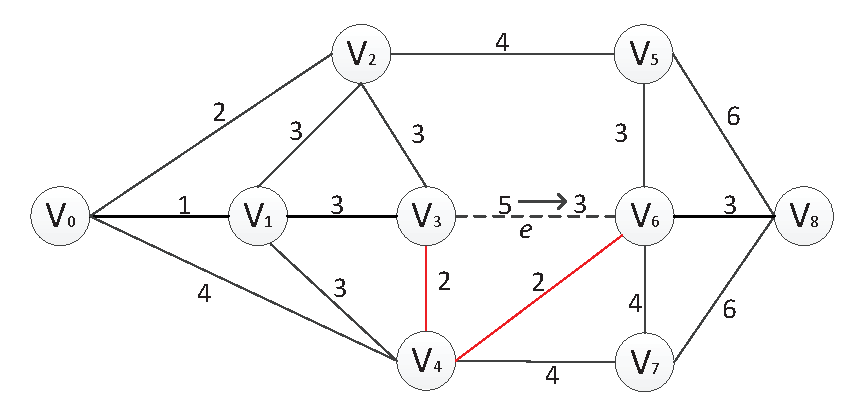
\includegraphics[scale=0.5]{figure/decrease.eps}
    \caption{An example of $w_e$ decreases.}
    \label{fig:decrease_example}
\end{figure}


Figure~\ref{fig:decrease_example} shows an example of computing affected paths on the graph when the weight of $e$ ($\langle v_3, v_6\rangle$) decreases from 5 to 3. Table~\ref{tab:algo1} shows the iteration process.

\begin{table}[htbp]
	\centering
	\caption{Iteration example of NEA.}
	\begin{tabular}{|l|l|l|l|l|l|}
    \hline
     & $C_s$ & $C_t$ & $v_s$ & $v_t$ & Affected paths \\
    \hline
    $1$ & $\{v3\}$ 		  & $\emptyset$ 	  & null & null &  \\
    $2$ & $\emptyset$	  & $\emptyset$       & $v3$ & null &  \\
    $3$ & $\emptyset$  & $\{v6\}$          & $v3$ & null &  \\
	$4$ & $\{v1,v2,v4\}$  & $\emptyset$ 	  & $v3$ & $v6$ &  \\
    $5$ & $\{v1,v2,v4\}$  & $\{v4,v5,v7,v8\}$ & $v3$ & $v6$ & $P_{3,6}$ \\
    $6$ & $\{v1,v2,v4\}$  & $\{v5,v7,v8\}$    & $v3$ & $v4$ & $P_{3,6}$ \\
    $7$ & $\{v1,v2,v4\}$  & $\{v7,v8,v2\}$ 	  & $v3$ & $v5$ & $P_{3,6},P_{3,5}$ \\
    $8$ & $\{v1,v2,v4\}$  & $\{v8,v2\}$ 	  & $v3$ & $v7$ & $P_{3,6},P_{3,5}$ \\
    $9$ & $\{v1,v2,v4\}$ & $\{v2\}$ 		  & $v3$ & $v8$ & $P_{3,6},P_{3,5},P_{3,8}$ \\
    $10$ & $\{v1,v2,v4\}$ & $\emptyset$ 	  & $v3$ & $v2$ & $P_{3,6},P_{3,5},P_{3,8}$ \\
    $11$ & $\{v2,v4\}$ 	  & $\emptyset$ 	  & $v1$ & $v6$ & $P_{3,6},P_{3,5},P_{3,8}$ \\
    $12$ & $\{v4\}$		  & $\emptyset$ 	  & $v2$ & $v6$ & $P_{3,6},P_{3,5},P_{3,8}$ \\
    $13$ & $\{v4,v0,v5\}$		  & $\{v4,v5,v7,v8\}$ & $v2$ & $v6$ & $P_{3,6},P_{3,5},P_{3,8},P_{2,6}$ \\
    $14$ & $...$		  & $...$ 	  &... & ... & ... \\
    $15$ & $\{v4,v0,v5\}$    & $\emptyset$ 	  & $v2$ & $v8$ & $P_{3,6},P_{3,5},P_{3,8},P_{2,6},P_{2,8}$ \\
    $16$ & $\{v0,v5\}$ 	  & $\emptyset$ 	  & $v4$ & $v6$ & $P_{3,6},P_{3,5},P_{3,8},P_{2,6},P_{2,8}$  \\
    $17$ & $\{v5\}$ 	  & $\emptyset$ 	  & $v0$ & $v6$ & $P_{3,6},P_{3,5},P_{3,8},P_{2,6},P_{2,8}$  \\
    $18$ & $\emptyset$ 	  & $\emptyset$ 	  & $v5$ & $v6$ & $P_{3,6},P_{3,5},P_{3,8},P_{2,6},P_{2,8}$  \\
    \hline
    \end{tabular}
    \label{tab:algo1}
\end{table}

\iffalse
\begin{table}[htbp]
	\centering
	\caption{Iteration example of NEA.}
	\begin{tabular}{|l|l|l|l|l|l|}
    \hline
     & $C_s$ & $C_t$ & $v_s$ & $v_t$ & $S_\textit{aff}$ \\
    \hline
    $1$ & $\{v3\}$ 		  & $\emptyset$ 	  & null & null &  \\
    $2$ & $\emptyset$	  & $\emptyset$       & $v3$ & null &  \\
    $3$ & $\emptyset$  & $\{v6\}$          & $v3$ & null &  \\
	$4$ & $\{v1,v2,v4\}$  & $\emptyset$ 	  & $v3$ & $v6$ &  \\
    $5$ & $\{v1,v2,v4\}$  & $\{v4,v5,v7,v8\}$ & $v3$ & $v6$ & $P_{3,6}$ \\
    $6$ & $\{v1,v2,v4\}$  & $\{v5,v7,v8\}$    & $v3$ & $v4$ & $P_{3,6}$ \\
    $7$ & $\{v1,v2,v4\}$  & $\{v7,v8,v2\}$ 	  & $v3$ & $v5$ & $P_{3,6},P_{3,5}$ \\
    $8$ & $\{v1,v2,v4\}$  & $\{v8,v2\}$ 	  & $v3$ & $v7$ & $P_{3,6},P_{3,5}$ \\
    $9$ & $\{v1,v2,v4\}$ & $\{v2\}$ 		  & $v3$ & $v8$ & $P_{3,6},P_{3,5},P_{3,8}$ \\
    $10$ & $\{v1,v2,v4\}$ & $\emptyset$ 	  & $v3$ & $v2$ & $P_{3,6},P_{3,5},P_{3,8}$ \\
    $11$ & $\{v2,v4\}$ 	  & $\emptyset$ 	  & $v1$ & $v6$ & $P_{3,6},P_{3,5},P_{3,8}$ \\
    $12$ & $\{v4\}$		  & $\emptyset$ 	  & $v2$ & $v6$ & $P_{3,6},P_{3,5},P_{3,8}$ \\
    $13$ & $\{v4\}$		  & $\{v4,v5,v7,v8\}$ & $v2$ & $v6$ & $P_{3,6},P_{3,5},P_{3,8},P_{2,6}$ \\
    $14$ & $...$		  & $...$ 	  &... & ... & ... \\
    $15$ & $\{v4,v5\}$    & $\emptyset$ 	  & $v2$ & $v8$ & $P_{3,6},P_{3,5},P_{3,8},P_{2,6},P_{2,8}$ \\
    $16$ & $\{v5\}$ 	  & $\emptyset$ 	  & $v4$ & $v6$ & $P_{3,6},P_{3,5},P_{3,8}$ \\
    $17$ & $\emptyset$ 	  & $\emptyset$ 	  & $v5$ & $v6$ & $P_{3,6},P_{3,5},P_{3,8}$ \\
    \hline
    \end{tabular}
    \label{tab:algo1}
\end{table}
\fi

\subsection{Outward Node Expansion Algorithm}
\label{sec:optimaization approaches}

In the above subsection, we introduce a basic method NEA to compute affected shortest paths when the weight of a certain edge decreases.
The above algorithm mainly has two components: which paths are detected and how to check whether they are affected.
In this part, we will present how to improve determining which paths are detected.

For ease of illustration, let $S_d(v_a)$ be the set of nodes whose node distance from $a$ is $d$.
%If a sequence $S=\langle v_a,v_1,...,vi,..,vn\rangle$ satisfies that the $i$th element $v_i\in S_i(v_a)$, we say it is an orderly sequence since the order of elements comply with the order of node distances.

\begin{corollary}
\label{thm:reduce-end-node}
Suppose the endpoints of $e$ are $v_a$ and $v_b$, and $v_i$ is an arbitrary node. If for any node $v_j \in S_d(v_b)$, $P_{i,j}$ does not contain $e$, then for any node $v_{j+1}\in S_{d+1}(v_b)$, one of the following stands: $S=\langle v_i,...,v_j,v_{j+1}\rangle$ is a shortest path and it does not contain $e$; $S$ is not a shortest path.
\end{corollary}
\begin{proof}
For any node $v_{j+1}\in S_{d+1}(v_b)$, if $P_{i,j+1}=\langle v_i,...,v_j,v_{j+1}\rangle$, $v_j\in S_d(v_b)$, and $P_{i,j}$ does not contain $e$, then according to Corollary~\ref{thm:node-node}, $P_{i,j+1}$ does not contain $e$.
\end{proof}

Recall the algorithm NEA, although start nodes are added to $C_s$ in a FIFO order i.e., nodes are expanded in a breath-first manner, the nodes in $C_s$ are not discriminated in terms of the node distance from $v_a$.
In this subsection, we expand nodes based on their distances from $v_a$. Thus, the algorithm is called outward node expansion algorithm (ONE).
An auxiliary set $C'_s$ is employed to store the nodes that are expanded from the nodes in $C_s$, therefore, $C_s=S_{d}(v_a)$ while $C'_s=S_{d+1}(v_a)$.

For a fixed node $v_a$, if a node $v_t$ satisfies that (1) $v_t$ is connected with $v_b$; and (2) $P'_{a,t}$ contains $e$, we add $v_t$ into $C_t$ (line~\ref{algo:2inis}-\ref{algo:2inie} of Algorithm~\ref{alg:comprising}).

\begin{algorithm}[htbp]
\small
\caption{{\textsc{Comprising $C_t$}} }
    \label{alg:comprising}
    \KwIn{A graph $G(V,E)$, the edge $e$ which decreases its weight and its endpoints $v_a$ and $v_b$, and a cache $\Psi$;}
    \KwOut{The set of termination nodes $C_t$;}
    add $v_b$ to $C_t$ and  $C'_t$\;\label{algo:2inis}
   \While{$C_t$ is not empty \&\& there are paths in $\Psi$ which are not checked}
        {
            $ v_t \leftarrow$  pop the first element from $C_t$\;
            calculate $P'_{a,t}$\;
            \If{ $P'_{a,t}$ contains $e$}{
                %$Found \leftarrow true$\;
                \If{$d(b,t)<K$}{
                    \For{each adjacent node $v_{adj}$ of $v_t$}{
                        \If{$v_{adj}$ has not been added into $C_t$ $\&\&$ $v_{adj}\neq v_a$}{
                            append $v_{adj}$ to $C_t$\;
                            append $v_{adj}$ to $C'_t$\;
                            }
                    }
                }
                \If{$P_{a,t}\in \Psi$}{
                    calculate $P_{a,t}$\;
                    \If{$P_{a,t} \neq P'_{a,t}$}{
                    delete $P_{a,t}$ from $\Psi$;
                    }
                    \Else {
                    mark ``checked'' for $P_{a,b}$;
                    }
                }
             }
             \ElseIf {$P_{a,b}\in \Psi$}{
             mark ``checked'' for $P_{a,b}$;
             }
        }\label{algo:2inie}
        \Return {$C_t$;}
\end{algorithm}

\begin{algorithm}[htbp]
\small
    \caption{\textsc{ONE}}
    \label{alg:candpath}
    \KwIn{A graph $G(V,E)$, the edge $e$ which decreases its weight and its endpoints $v_a$ and $v_b$, and a cache $\Psi$;}
    \KwOut{The cache $\Psi$ after deletion of affected paths;}
    Comprising $C_t$;
    replace $C_t$ with $C'_t$\;
    \For{each adjacent node $v_{adj}$  of  $v_a$}{
        add $v_{adj}$ to $C_s$\;
    }
    \While{$C_s$ is not empty \&\& there are paths in $\Psi$ which are not checked}{
        $C'_s \leftarrow \emptyset$;
        $C'_t \leftarrow \emptyset$; \tcp{initialize auxiliary sets}

        \For{ each node $v_s$ in $C_s$}{
           calculate $P'_{s,b}$\;
            \If{ $P'_{s,b}$ contains $e$}{\label{algo:2conte}
                \If {$d'(s,a)<K$}{
                    \For{each adjacent node $v_{adj}$  of  $v_s$}{
                        \If{ $v_{adj}$ has not been added into $C_s$ $\&\&$ $v_{adj}\neq v_b$}{
                            add $v_{adj}$ to $C'_s$; \tcp{store $v_{adj}$ for the next round}
                        }
                    }
                }
            }
            \For{ each $v_t$ in ${C_t}$}{\label{algo:2forvt}
                calculate $P'_{s,t}$\;
                \If{ $P'_{s,t}$ contains $e$}{
                    add $v_t$ to $ C'_t$; \tcp{store $v_t$ for the next round}
                    \If{$P_{s,t}\in \Psi$}{
                        calculate $P_{s,t}$\; \label{algo:2calPse}
                        \If{$P_{s,t} \neq P'_{s,t}$} {\label{algo:2unequal}
                            delete $P_{s,t}$ from $\Psi$;\label{algo:2end}
                        }
                        \Else {
                        mark ``checked'' for $P_{s,t}$;
                        }
                    }
                }
                \ElseIf {$P_{s,t}\in \Psi$}{
                mark ``checked'' for $P_{s,t}$;
                }
            }
        }
    }
    replace $C_s$ and  $C_t$  with $C'_s $ and $C'_t$, respectivley\;
    \Return{$\Psi$;}
\end{algorithm}


Starting from iteration $d=1$, we try to reduce the size of $C_t$.
For a node $v_t\in C_t$, if $P'_{s,t}$ does not contain $e$ for any node $v_s\in S_{d}(v_a)$, then according to Corollary~\ref{thm:reduce-end-node}, $P'_{s,t}$ does not contain $e$ for any node $v_s\in S_{d+1}(v_a)$.
Therefore, $v_t$ is deleted from $C_t$, reflecting by not being added into $C'_t$.
Hence, ONE saves the time of visiting $v_t$ in the $d+1$th (and latter iterations) and calculating corresponding shortest paths.

Based on ONE, the iteration process of example Figure~\ref{fig:decrease_example} is displayed in Table~\ref{tab:algo2}.
\begin{table}[htbp]
	\centering
	\caption{Iteration example of ONE.}
	\begin{tabular}{|l|l|l|l|l|l|}
    \hline
     & $C_s$ & $C_t$ & $v_s$ & $v_t$ & Affected paths \\
    \hline
    $1$ & $\{v3\}$ 		  & $\emptyset$ 	  & null & null &  \\
    $2$ & $\emptyset$	  & $\emptyset$       & $v3$ & null &  \\
    $3$ & $\emptyset$  & $\{v6\}$          & $v3$ & null &  \\
	$4$ & $\{v1,v2,v4\}$  & $\emptyset$ 	  & $v3$ & $v6$ &  \\
    $5$ & $\{v1,v2,v4\}$  & $\{v4,v5,v7,v8\}$ & $v3$ & $v6$ & $P_{3,6}$ \\
    $6$ & $\{v1,v2,v4\}$  & $\{v5,v7,v8\}$    & $v3$ & $v4$ & $P_{3,6}$ \\
    $7$ & $\{v1,v2,v4\}$  & $\{v2,v7,v8\}$ 	  & $v3$ & $v5$ & $P_{3,6},P_{3,5}$ \\
    $8$ & $\{v1,v2,v4\}$  & $\{v7,v8\}$ 	  & $v3$ & $v2$ & $P_{3,6},P_{3,5}$ \\
    $9$ & $\{v1,v2,v4\}$ & $\{v8\}$ 		  & $v3$ & $v7$ & $P_{3,6},P_{3,5}$ \\
    $10$ & $\{v1,v2,v4\}$ & $\emptyset$ 	  & $v3$ & $v8$ & $P_{3,6},P_{3,5},P_{3,8}$ \\
    $11$ & $\{v2,v4\}$ 	  & $\emptyset$ 	  & $v1$ & $v6$ & $P_{3,6},P_{3,5},P_{3,8}$ \\
    $12$ & $\{v4\}$		  & $\{v6,v5,v8\}$ 	  & $v2$ & $null$ & $P_{3,6},P_{3,5},P_{3,8}$ \\
    $13$ & $\{v4,v0,v5\}$		  & $\{v5,v8\}$ 	      & $v2$ & $v6$ & $P_{3,6},P_{3,5},P_{3,8},P_{2,6}$ \\
    $14$ & $\{v4,v0,v5\}$		  & $\{v8\}$ 	      & $v2$ & $v5$ & $P_{3,6},P_{3,5},P_{3,8},P_{2,6}$ \\
    $15$ & $\{v4,v0,v5\}$		  & $\emptyset$ 	  & $v2$ & $v8$ & $P_{3,6},P_{3,5},P_{3,8},P_{2,6},P_{2,8}$ \\
    $16$ & $\{v0,v5\}$ 	  & $\emptyset$ 	  & $v4$ & $v6$ & $P_{3,6},P_{3,5},P_{3,8},P_{2,6},P_{2,8}$\\
    $17$ & $\{v5\}$ 	  & $\emptyset$ 	  & $v0$ & $v6$ & $P_{3,6},P_{3,5},P_{3,8},P_{2,6},P_{2,8}$\\
    $18$ & $\emptyset$ 	  & $\emptyset$ 	  & $v5$ & $v6$ & $P_{3,6},P_{3,5},P_{3,8},P_{2,6},P_{2,8}$ \\
    \hline
    \end{tabular}
    \label{tab:algo2}
\end{table}

\iffalse
\begin{table}[htbp]
	\centering
	\caption{Iteration example of ONE.}
	\begin{tabular}{|l|l|l|l|l|l|}
    \hline
     & $C_s$ & $C_t$ & $v_s$ & $v_t$ & $S_\textit{aff}$ \\
    \hline
    $1$ & $\{v3\}$ 		  & $\emptyset$ 	  & null & null &  \\
    $2$ & $\emptyset$	  & $\emptyset$       & $v3$ & null &  \\
    $3$ & $\emptyset$  & $\{v6\}$          & $v3$ & null &  \\
	$4$ & $\{v1,v2,v4\}$  & $\emptyset$ 	  & $v3$ & $v6$ &  \\
    $5$ & $\{v1,v2,v4\}$  & $\{v4,v5,v7,v8\}$ & $v3$ & $v6$ & $P_{3,6}$ \\
    $6$ & $\{v1,v2,v4\}$  & $\{v5,v7,v8\}$    & $v3$ & $v4$ & $P_{3,6}$ \\
    $7$ & $\{v1,v2,v4\}$  & $\{v2,v7,v8\}$ 	  & $v3$ & $v5$ & $P_{3,6},P_{3,5}$ \\
    $8$ & $\{v1,v2,v4\}$  & $\{v7,v8\}$ 	  & $v3$ & $v2$ & $P_{3,6},P_{3,5}$ \\
    $9$ & $\{v1,v2,v4\}$ & $\{v8\}$ 		  & $v3$ & $v7$ & $P_{3,6},P_{3,5}$ \\
    $10$ & $\{v1,v2,v4\}$ & $\emptyset$ 	  & $v3$ & $v8$ & $P_{3,6},P_{3,5},P_{3,8}$ \\
    $11$ & $\{v2,v4\}$ 	  & $\emptyset$ 	  & $v1$ & $v6$ & $P_{3,6},P_{3,5},P_{3,8}$ \\
    $12$ & $\{v4\}$		  & $\{v6,v8\}$ 	  & $v2$ & $null$ & $P_{3,6},P_{3,5},P_{3,8}$ \\
    $13$ & $\{v4\}$		  & $\{v8\}$ 	      & $v2$ & $v6$ & $P_{3,6},P_{3,5},P_{3,8},P_{2,6}$ \\
    $14$ & $\{v4\}$		  & $\emptyset$ 	  & $v2$ & $v8$ & $P_{3,6},P_{3,5},P_{3,8},P_{2,6},P_{2,8}$ \\
    $15$ & $\{v5\}$ 	  & $\emptyset$ 	  & $v4$ & $v6$ & $P_{3,6},P_{3,5},P_{3,8}$ \\
    $16$ & $\emptyset$ 	  & $\emptyset$ 	  & $v5$ & $v6$ & $P_{3,6},P_{3,5},P_{3,8}$ \\
    \hline
    \end{tabular}
    \label{tab:algo2}
\end{table}
\fi


\subsection{Inward Node Expansion Algorithm}

In this section, we present another two techniques to improve the efficiency of affected shortest path detection.
\begin{corollary}
\label{thm:check}
Suppose the end nodes of $e$ are $v_a$ and $v_b$. When $w_e$ decreases, if $P_{a,b}$ is an affected path, then any shortest path $P'_{s,t}$ which contains $e$ is an affected path, i.e., $P'_{s,t} \neq P_{s,t}$.
\end{corollary}


\begin{proof}
Assume that there exists a path $P'_{s,t}$ which contains $e$ and $P_{s,t}=P'_{s,t}$.
As $P_{a,b}$ is an affected shortest path, we know $P_{a,b}=S1=\langle v_a,v_m,...,v_n,v_b\rangle$ and $P'_{a,b}=S2=\langle v_a,v_b\rangle=e$ and $w'_{S2}<w'_{S1}=w_{S1}<w_{S2}$.
Since $P'_{s,t}$ contains $e$, the sequence of $P'_{s,t}$ must be $S3=\langle v_s,...,v_a,v_b,...,v_t\rangle $. If we substitute $\langle v_a,v_b\rangle$ ($S2$) in $S3$ with $S1$, we have $S4=\langle v_s,...,v_a,v_m,...,v_n,v_b,...,v_t\rangle$. It is clearly that $w_{S4}<w_{S3}$, therefore $P_{s,t}$ can not be $S3$. The assumption does not hold; therefore our corollary stands.
\end{proof}

According to Corollary~\ref{thm:check}, the process of detecting whether a path is affected is shortened. If $P_{a,b}$ is an affected shortest path, we can avoid the calculation of $P_{s,t}$ in line~\ref{algo:2calPse} and comparison with $P'_{a,b}$ in line~\ref{algo:2unequal} of Algorithm~\ref{alg:candpath}.
Since $P'_{s,t}$ contains $e$ (line~\ref{algo:2conte} of Algorithm~\ref{alg:candpath}), so we can know $P_{s,t}$ is an affected path directly.

We now focus on the order of generating node-pairs with each from $C_s$ and $C_t$, respectively.

\begin{corollary}
\label{thm:longer}
Suppose $v_a$ and $v_b$ are endpoints of $e$, $v_s$ ($v_t$) is a node connected with $v_a$ ($v_b$). If $P_{s,t}$ contains $e$, then for a node $v_k$ after $v_b$ in the sequence of $P_{s,t}$, at least one path of $P_{s,k}$ contains $e$.
\end{corollary}

\begin{proof}
Since $P_{s,t}$ is a shortest path, its subpath $\langle v_s,...,v_a,v_b,...,v_k\rangle $ is also a shortest path, i.e., $P_{s,k}=\langle v_s,...,v_a,v_b,...,v_k\rangle$ and $P_{s,k}$ contains $e$.
\end{proof}

Corollary~\ref{thm:longer} tells us that for a node $v_s$ connected with $v_a$, if a path $P_{s,t}$ ($v_t\in S_{d}(v_b)$) contains $e$, then $P'_{s,k}$ ($v_k$ is on $P'_{s,t}=\langle v_s,...,v_a,v_b,...,v_k,...v_t\rangle$) contains $e$ as well. It is not necessary to compute $P'_{s,k}$ and compare it with $P_{s,k}$. Therefore, for a fixed $v_s$ from $C_s$, we should prioritize $v_t$ with large $d_{b,t}$ to comprise a node pair.

We have an optimized algorithm-inward node expansion algorithm (INE). The term ``inward'' stems from that fact that nodes of $C_t$ are visited from far nodes to close nodes, at last $v_b$.
Since the main logic of INE is the same with ONE, we only demonstrate different lines. INE replaces line~\ref{algo:2forvt}-\ref{algo:2end} of ONE with the code in Algorithm~\ref{alg:candpathplus}.



\begin{algorithm}[htbp]
{\small
     \caption{{\textsc{INE}} }
    \label{alg:candpathplus}
      \While{$C_t$ is not empty}{
          $v_t  \leftarrow $ pop the node in $C_t$ which has the largest node distance from $v_b$\;
          calculate $P'_{s,t}$\;
          \If{ $P'_{s,t}$ contains $e$}{
                \For{ each $v_k$ lies on path $P'_{s,t}$ $\&\&$ $v_k$ is after $v_b$}{
                   add $v_k$ into $C'_t$\; \label{algo:3add}
                   pop $v_k$ from ${C_t}$\;\label{algo:3pop}
                \If{ $P_{a,b}$ is an affected path \&\& $P_{a,b}\in \Psi$}
                {\label{algo:3ifpab}
                     delete $P_{s,k}$ from $\Psi$\;
                }
                \ElseIf {$P_{s,t}\in \Psi$}{
                    calculate  $P_{s,k}$\;
                    \If{$P_{s,k} \neq P'_{s,k}$}{
                    delete $P_{s,k}$ from $\Psi$\;
                    }
               }

          }
        }
        \ElseIf{$P_{s,t}\in \Psi$} {
        mark ``checked'' for $P_{s,t}$;
        }
     }
}
\end{algorithm}

In Algorithm~\ref{alg:candpathplus}, line~\ref{algo:3add}-\ref{algo:3pop} indicate that if $v_k$ is on a shortest path which contains $e$, then $P'_{s,k}$ must contain $e$, therefore $v_k$ is added into $C'_t$ for the next iteration directly without computing $P'_{s,k}$. The IF sentence in line~\ref{algo:3ifpab} makes use of Corollary~\ref{thm:check}.



Take Figure~\ref{fig:decrease_example} as an example, the iteration process by INE is illustrated in Table~\ref{tab:algo3}.
\begin{table}[htbp]
	\centering
	\caption{Iteration example of INE.}
	\begin{tabular}{|l|l|l|l|l|l|}
    \hline
     & $C_s$ & $C_t$ & $v_s$ & $v_t$ & Affected paths \\
    \hline
    $1$ & $\{v3\}$ 		  & $\emptyset$ 	  & null & null &  \\
    $2$ & $\emptyset$	  & $\emptyset$       & $v3$ & null &  \\
    $3$ & $\emptyset$  & $\{v6\}$          & $v3$ & null &  \\
	$4$ & $\{v1,v2,v4\}$  & $\emptyset$ 	  & $v3$ & $v6$ &  \\
    $5$ & $\{v1,v2,v4\}$  & $\{v4,v5,v7,v8\}$ & $v3$ & $v6$ & $P_{3,6}$ \\
    $6$ & $\{v1,v2,v4\}$  & $\{v5,v7,v8\}$    & $v3$ & $v4$ & $P_{3,6}$ \\
    $7$ & $\{v1,v2,v4\}$  & $\{v2,v7,v8\}$ 	  & $v3$ & $v5$ & $P_{3,6},P_{3,5}$ \\
    $8$ & $\{v1,v2,v4\}$  & $\{v7,v8\}$ 	  & $v3$ & $v2$ & $P_{3,6},P_{3,5}$ \\
    $9$ & $\{v1,v2,v4\}$ & $\{v8\}$ 		  & $v3$ & $v7$ & $P_{3,6},P_{3,5}$ \\
    $10$ & $\{v1,v2,v4\}$ & $\emptyset$ 	  & $v3$ & $v8$ & $P_{3,6},P_{3,5},P_{3,8}$ \\
    $11$ & $\{v2,v4\}$ 	  & $\emptyset$ 	  & $v1$ & $v6$ & $P_{3,6},P_{3,5},P_{3,8}$ \\
    $12$ & $\{v4\}$		  & $\{v6,v5,v8\}$ 	      & $v2$ & $null$ & $P_{3,6},P_{3,5},P_{3,8}$ \\
    $13$ & $\{v4\}$		  & $\{v5\}$ 	  & $v2$ & $v8$ & $P_{3,6},P_{3,5},P_{3,8},P_{2,6},P_{2,8}$ \\
    $14$ & $\{v4,v0,v5\}$		  & $\emptyset$ 	  & $v2$ & $v5$ & $P_{3,6},P_{3,5},P_{3,8},P_{2,6},P_{2,8}$ \\
    $15$ & $\{v0,v5\}$ 	  & $\emptyset$ 	  & $v4$ & $v6$ & $P_{3,6},P_{3,5},P_{3,8},P_{2,6},P_{2,8}$  \\
     $16$ & $\{v5\}$ 	  & $\emptyset$ 	  & $v0$ & $v6$ & $P_{3,6},P_{3,5},P_{3,8},P_{2,6},P_{2,8}$  \\
    $17$ & $\emptyset$ 	  & $\emptyset$ 	  & $v5$ & $v6$ & $P_{3,6},P_{3,5},P_{3,8},P_{2,6},P_{2,8}$  \\
    \hline
    \end{tabular}
    \label{tab:algo3}
\end{table}

\iffalse
\begin{table}[htbp]
	\centering
	\caption{Iteration example of INE.}
	\begin{tabular}{|l|l|l|l|l|l|}
    \hline
     & $C_s$ & $C_t$ & $v_s$ & $v_t$ & $S_\textit{aff}$ \\
    \hline
    $1$ & $\{v3\}$ 		  & $\emptyset$ 	  & null & null &  \\
    $2$ & $\emptyset$	  & $\emptyset$       & $v3$ & null &  \\
    $3$ & $\emptyset$  & $\{v6\}$          & $v3$ & null &  \\
	$4$ & $\{v1,v2,v4\}$  & $\emptyset$ 	  & $v3$ & $v6$ &  \\
    $5$ & $\{v1,v2,v4\}$  & $\{v4,v5,v7,v8\}$ & $v3$ & $v6$ & $P_{3,6}$ \\
    $6$ & $\{v1,v2,v4\}$  & $\{v5,v7,v8\}$    & $v3$ & $v4$ & $P_{3,6}$ \\
    $7$ & $\{v1,v2,v4\}$  & $\{v2,v7,v8\}$ 	  & $v3$ & $v5$ & $P_{3,6},P_{3,5}$ \\
    $8$ & $\{v1,v2,v4\}$  & $\{v7,v8\}$ 	  & $v3$ & $v2$ & $P_{3,6},P_{3,5}$ \\
    $9$ & $\{v1,v2,v4\}$ & $\{v8\}$ 		  & $v3$ & $v7$ & $P_{3,6},P_{3,5}$ \\
    $10$ & $\{v1,v2,v4\}$ & $\emptyset$ 	  & $v3$ & $v8$ & $P_{3,6},P_{3,5},P_{3,8}$ \\
    $11$ & $\{v2,v4\}$ 	  & $\emptyset$ 	  & $v1$ & $v6$ & $P_{3,6},P_{3,5},P_{3,8}$ \\
    $12$ & $\{v4\}$		  & $\{v8\}$ 	      & $v2$ & $null$ & $P_{3,6},P_{3,5},P_{3,8}$ \\
    $13$ & $\{v4\}$		  & $\emptyset$ 	  & $v2$ & $v8$ & $P_{3,6},P_{3,5},P_{3,8},P_{2,6},P_{2,8}$ \\
    $14$ & $\{v5\}$ 	  & $\emptyset$ 	  & $v4$ & $v6$ & $P_{3,6},P_{3,5},P_{3,8}$ \\
    $15$ & $\emptyset$ 	  & $\emptyset$ 	  & $v5$ & $v6$ & $P_{3,6},P_{3,5},P_{3,8}$ \\
    \hline
    \end{tabular}
    \label{tab:algo3}
\end{table}
\fi

Now we compare the performance of three algorithms. The nodes visited by the three proposed algorithms are displayed in Table~\ref{tab:algocomp}.
The numbers of nodes visited satisfy NEA$>$ONE$>$INE, and the numbers of iterations are still NEA$>$ONE$>$INE.
\begin{table}[htbp]
	\centering
	\caption{Performance comparison of algorithms.}
	\begin{tabular}{|l|l|l|l|l|}
    \hline
     & $v_s$ & $C_t$ (NEA) & $C_t$ (ONE) & $C_t$ (INE)  \\
    \hline
    $1$ & $v3$   & $\{v2,v4,v5,v6,v7,v8\}$	  & $\{v2,v4,v5,v6,v7,v8\}$	& $\{v2,v4,v5,v6,v7,v8\}$	 \\
    $2$ & $v1$   & $\{v6\}$	 &  $\{v6\}$	&  $\{v6\}$ \\
     $3$ & $v2$   & $\{v4,v5,v6,v7,v8\}$	 & $\{v5,v6,v8\}$& $\{v5,v8\}$	 \\
     $4$ & $v4$   & $\{v6\}$	 & $\{v6\}$	& $\{v6\}$	 \\
      $5$ & $v0$   & $\{v6\}$	 & $\{v6\}$	& $\{v6\}$ \\
     $6$ & $v5$   & $\{v6\}$	 & $\{v6\}$	& $\{v6\}$ \\
    \hline
    \end{tabular}
    \label{tab:algocomp}
\end{table}
\iffalse
\begin{table}[htbp]
	\centering
	\caption{Performance comparison of algorithms.}
	\begin{tabular}{|l|l|l|l|l|}
    \hline
     & $v_s$ & $C_t$(NEA) & $C_t$(ONE) & $C_t$(INE)  \\
    \hline
    $1$ & $v3$   & $\{v2,v4,v5,v6,v7,v8\}$	  & $\{v2,v4,v5,v6,v7,v8\}$	& $\{v2,v4,v5,v6,v7,v8\}$	 \\
    $2$ & $v1$   & $\{v6\}$	 &  $\{v6\}$	&  $\{v6\}$ \\
     $3$ & $v2$   & $\{v4,v5,v6,v7,v8\}$	 & $\{v6,v8\}$& $\{v8\}$	 \\
     $3$ & $v4$   & $\{v6\}$	 & $\{v6\}$	& $\{v6\}$	 \\
     $3$ & $v5$   & $\{v6\}$	 & $\emptyset$	& $\emptyset$ \\
    \hline
    \end{tabular}
    \label{tab:algocomp}
\end{table}
\fi

%In terms of the time complexity, NEA computes all node-pairs with each from $C_s$ and $C_t$, respectively. For a graph with $N$ nodes, the time complexity is $\mathcal O(N^2)$.
%ONE and INE are improved on the basis of NEA. However, in the worst case, the start and termination sets include all nodes. Thus, the time complexity of two optimized algorithms are still $\mathcal O(N^2)$.



\section{Refreshment Strategies}
\label{sec:strategies}

In this section, we introduce four heuristic-based cache refreshment strategies.

\subsection{Reload Whole Cache}

The first refreshment strategy is to empty the whole cache and reload it based on benefit values. The strategy is abbreviated as RWC.
This is the most straightforward idea to refresh the cache.
The benefit value is proposed in \cite{Li2014refreshment}. To make this paper self-contained, we briefly introduce how the benefit oriented model works.

All of us know that the cache utilization, or the cost reduction by using cache, is affected by the query frequency and the computational time of shortest paths. When calculating the cost saved by loading a path $P_{i,j}$ into a cache, we consider: 1) which queries can be answered by $P_{i,j}$ ; and 2) the saved computational cost if answering a query $Q_{i,j}$ by a cache directly.

For the first consideration, we know that a path can answer all the queries on its subpaths~\citep{cormen2001introduction}.
For the second consideration, it depends on how frequently a query arrives and the computational cost of that query. More specifically, it is the multiplier of the query frequency and the computational cost.

From the above analysis, the utilization of storing $P_{i,j}$ into a cache is:
\begin{equation}
B(P_{i,j},\Psi)= \frac{\sum_{P_{s,t} \in S(P_{i,j})\& P_{s,t}\notin S(\Psi)} {F_{s,t}}\cdot C_{s,t}}{|P_{i,j}|}.
\end{equation}

Here, $S(P_{i,j})$ is the set of subpaths of $P_{i,j}$, and the numerator is the total cost reduction saved by caching path $P_{i,j}$. After normalized by the size of $P_{i,j}$, $B(P_{i,j})$ is the unit-size benefit brought by loading $P_{i,j}$ into a cache.
Readers can understand this as the value of per unit weight in a knapsack problem. Paths with larger $B(P_{i,j})$ have higher priority to be loaded into a cache.
When the cache is placed at the proxy, the time of computing shortest paths mainly lies on the round-trip communication time, which is the same for all queries \citep{thomsen2012effective}.

Suppose the number of nodes in graph $G$ is $N$, the size of query log is $|L|$, the number of paths in the path array is $m$, the number of node vector in the bitmap is $n$. For the RWC, all shortest paths queried in the query log are computed. The time complexity is $\mathcal O(|L|*N^2)$. The benefit values of shortest paths are computed and sorted. The complexity of such actions are $\mathcal O(|L|\log |L|)$. The time complexity of constructing path array and bitmap is $\mathcal O(m+n)$. The time complexity of this algorithm is $\mathcal O(|L|*N^2+|L|\log |L|+m+n)$.


\subsection{Update Affected Shortest Paths}

The first method wastes a lot of time. Since only an edge changes its weight, its impact on the whole network is limited. The majority of shortest paths do not change at all. As a result, reloading the whole cache is redundant. To overcome the shortcoming of the first method, we update all the affected paths in the cache.
If the size of affected paths exceed the available space of the cache, shortest paths with the largest benefit values are loaded into the cache.

Suppose the number of nodes in graph $G$ is $N$, the size of query log is $|L|$, the number of paths in the path array is $m$, the number of node vector in the bitmap is $n$.
The time complexity of affected shortest paths detection is $\mathcal O(N^2)$. In the worst case, all paths in the cache are updated. Therefore, the time complexity of updating affected shortest paths is $\mathcal O(m*N^2)$. The time complexity of sorting benefit values of affected shortest paths is $\mathcal O(m\log m)$. The complexity of UASP
\subsection{Replace Affected Paths with Highest Frequency Paths}

The above method need update benefit values of affected paths.
In the third method, after we delete the affected paths we fill the cache with paths which have the highest query frequencies. Query frequencies, instead, can be easily obtained from the query log and never change even though the network changes. It avoids computing the benefit of each path but it takes time to sort frequencies.


\subsection{Replace Affected Paths Using Roulette Wheel Selection}

At last, the fourth strategy is to delete all the affected paths in the cache and load new paths to the cache by the method of \emph{roulette wheel}. As the historical queries are not the true queries in the future, on one hand, we consider it as a reference for the future queries; on the other hand, we avoid over fitting the cache content to it.

We use a roulette wheel to determine which paths should be loaded into the cache. One feature of the roulette wheel selection is that alternatives with low attractiveness can also be selected, although with a relatively low possibility. We adopt the idea of roulette wheel as follows: for a path $p$ in the query log, its probability of being selected $\Pr(p)$ is proportional to its query frequency $f_p$, as shown in Equation~\ref{eq:RWS-probalibity}.

\begin{equation}
\label{eq:RWS-probalibity}
\Pr(p)= \frac{f_p}{\sum_{i} {f_i}}.
\end{equation}

The summation of the probabilities of all the paths is 1. The probability of selecting each path corresponds to the probability of a variable $X$ with a standard uniform distribution falling into an interval as shown in Equation~\ref{eq:RWS-range}.

\begin{equation}
\label{eq:RWS-range}
\Pr(p) = \Pr(X\in[\frac{\sum_{i=1}^{p-1}{f_i}}{\sum_i f_i},\frac{\sum_{i=1}^{p}{f_i}}{\sum_i f_i}]).
\end{equation}
In another word, to realize the probabilities for all the paths is equivalent to generate a random number which falls at interval [0, 1].

Take Table~\ref{tab:refresh-example} for example, it records the path-interval correspondence. When we need to select a path into the cache, we generate a random number according to a standard uniform distribution.
Suppose the randomly generated number is 0.6, then $P_{2,11}$ will be selected because 0.6 belongs to $[0.5,0.75]$.

\begin{table}[thbp]
\caption{A example of roulette wheel selection.}
\centering
\label{tab:refresh-example}
\begin{tabular}{|l|c|c|l|}
\hline
Path             & Frequency & Probability & Interval\\
\hline
$P_{1,12}$       &6          &0.3          &$[0,0.3]$\\
$P_{1,10}$       &3          &0.15         &$[0.3,0.45]$\\
$P_{6,9}$        &1          &0.05         &$[0.45,0.5]$\\
$P_{2,11}$       &5          &0.25         &$[0.5,0.75]$\\
$P_{1,8}$        &2          &0.1          &$[0.75,0.85]$\\
$P_{7,12}$       &3          &0.15         &$[0.85,1.0]$\\
\hline
\end{tabular}
\end{table}

%In terms of the computational time, the replace affected paths using roulette wheel selection is slower than the reload affected paths  and the replace affected paths with highest frequency faster than the reload whole cache. As for the performance, it is better than the former two and worse than the reload whole cache. Choosing which refreshment strategy is based on the scenario requirement. When time is not a concern, then the reload whole cache or the replace affected paths using roulette wheel selection may be used; When real time response is a big issue, the reload affected paths or the replace affected paths with highest frequency may be utilized. There is no absolutely good or absolutely bad.

%\iffalse
%\usepackage{array}
%|p{2cm}<{\centering}|
%\fi


%Algorithm~\ref{alg:selecthigh} describes the process of selecting paths from query log. To begin with, affected paths in cache are deleted, and the algorithm then sort the paths in query log according to their frequencies in descending order. When the query is not in cache, its corresponding shortest path is computed, and will be loaded in when it��s smaller than the remaining space ($\Omega-|\Psi|$) in cache.
%
%\begin{algorithm}[htbp]
%{\small
%    \caption{{\textsc{SelectHighFreq}} }
%    \label{alg:selecthigh}
%    Remove Saff from Csys\;
%    Rank query log Clog with frequency\;
%
%  \For{each query $Q_i$ in $C_{log}$}{
%  \If{ $Q_i \notin C_{log}$ and $|Q_i|\leq \Omega-|\Psi|$}{
%    $P_i \leftarrow$ Calculate the shortest path of $Q_i$ \;
%    $C_{sys} \leftarrow P_i$\;
%  }
%  \Else{
%    \Return;
%  }
%  }
%}
%\end{algorithm}

%For instance, for the query shown in Table~\ref{tab:refresh-example}, according to highest frequency guided rule, the order of selected query would be: $Q_{1,12}$,$Q_{2,11}$,$Q_{1,10}$,$Q_{7,12}$,$Q_{1,8}$,$Q_{6,9}$, and if current space in cache can contain 12 nodes, then $Q_{1,12}$,$Q_{2,11}$ will be added into cache.

%\section{Cache Structure}
%\label{sec:structure}

\textbf{Discussion}. In terms of the computational time, reloading the whole cache apparently costs the most time. Replacing affected paths with the highest frequency costs the second since it takes time to sort the frequencies of all shortest paths. Replacing affected paths using roulette wheel selection ranks the third, since it has a process of roulette wheel selection. Replacing affected paths using the largest benefit values costs the least time since only a small set of affected paths update their benefit values.









\section{Experiments }
\label{sec:exp}

We used three data sets Aalborg\footnote{http://www.dbxr.org/experimental-guidelines/}, Beijing\footnote{http://arxiv.org/abs/cs/04100001}, and Singapore \citep{Song2014PRESS} in our experiments. Each data set consists of a weighted road network and a query log. Since the numbers of queries in the Aalborg and Beijing query logs are relatively small, we enlarge the query logs.
The query log of each data set is divided into two parts; one half is the training set and the other half is the test set. Training sets act as historical logs while test sets act as future queries. The frequency statistics are extracted from the training set, and the cache is filled based on benefit values.
Table \ref{tab:datasetinfo} summarizes the information on the data sets. Columns ``Size of training set'' and ``Size of test set'' indicate the number of queries in the training set and test set, respectively. We assume that the query trend on training sets and test sets are similar, and the statistic information from training sets can predict future queries to some extent.

 \begin{table}[htbp]
 \caption{Information of data sets.}
 \centering
 \label{tab:datasetinfo}
{
 \begin{tabular}{c|c|c|c|c}
 \hline
  Data set   & No. of nodes & No. of edges & Size of training set & Size of test set\\
  \hline
  Aalborg    & 129k         & 137k         &23,720                            & 23,720\\
  \hline
   Beijing   & 76k          &85k           &64,640                            & 64,640\\
  \hline
   Singapore & 20,801       &55,892        &150,000                           & 150,000\\
   \hline
 \end{tabular}
}
\end{table}

We generated 50 instances based on each data set; one half of the instances increase weights of edges and the other half decrease weights. The increased and decreased edges must a relatively high impact on the response efficiency.
To meet the criteria, we firstly generated instances with weights increased, then the decreased instances. Hereafter, we explain the process of generating instances for Aalborg. For the other data sets, the process is totally the same.

The cache was initialized based on the road network and training set of Aalborg.
For each path in the cache, two consecutive nodes of the path forms an edge. We sorted all edges formed by the cached paths based on edges' frequencies of appearance. The 25 edges with the highest frequencies were marked.
The road network in Aalborg act as the road network before the weight of one edge is increased (original network). Each time, we selected one marked edge $e$ and increased $w_e$ by 10 times, resulting in a changed road network (new network). The 25 edges were sequentially increased and 25 corresponding instances with weights increased were obtained.
For the instances of weights decreased, new networks of increased instances act as the original networks. When $w_e$ of marked edges recovered to their weights recorded in Aalborg, we yielded instances with decreased weights.


All the code was implemented in GNU C++. The experiments were run on a PC with an Intel i7 Quad Core CPU clocked at 3.10 GHz.

\subsection{Effect of Cache Structure}
\label{sec:effect-cache-structure}
We use a bitmap-based structure in Section~\ref{sec:Cache Structure} to facilitate the cache on answering users' queries.
To have an impression of how the bitmap structure works, we compare it with a benchmark structure, which only records shortest paths in a path array.
Queries are answered by scanning the array.
The benchmark structure is called a basic cache.

For each data set, the cache is firstly initialized based on the largest benefit values of paths in the query log. Queries in the test sets arrive one by one and the total response time by two cache structure is displayed in Figure~\ref{fig:time-cache-structure}. We can see that the time performance of bitmap structure is much better than that of basic structure. The response time of bitmap is only 0.7ms when the cache size is 9MB for the Aalborg data set, while it costs 205ms for the basic structure. We can get consistent results on Beijing and Singapore data sets.
Moreover, the response time is almost constant with the increase of cache size for the bitmap structure.
\begin{figure}[htbp]
\centering
    \subfigure[{\footnotesize Aalborg}]
   {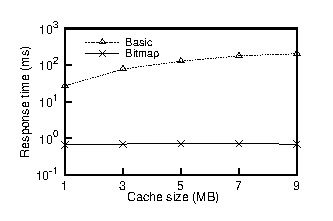
\includegraphics
   [height=3.5cm]{figure/construct-cache-time-aal.eps}}
   \subfigure[{\footnotesize Beijing}]
   {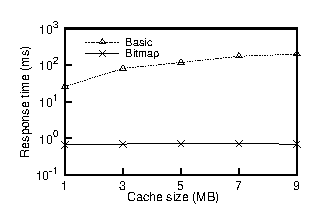
\includegraphics [height=3.5cm]{figure/construct-cache-time-beijing.eps}}
   \subfigure[{\footnotesize Singapore}]
   {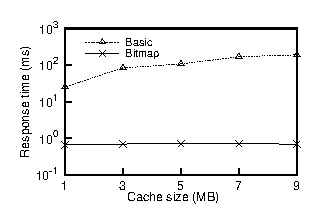
\includegraphics [height=3.5cm]{figure/construct-cache-time-singapore.eps}}
 \caption{Response time of cache structures.}
 \label{fig:time-cache-structure}
\end{figure}


\subsection{Efficiency of Detecting Affected Paths in the Cache}
\label{ssec:efficiency-detecting}
Detecting affected paths in a cache is an important step before refreshing a cache. To demonstrate the performance of our algorithms, a naive method (NM) is used as a benchmark method. Due to the size of graph, NM only re-computes new shortest paths for all pairs of nodes in the cache and compares them with the original ones. If the two shortest paths for a pair of nodes are different, then an affected path is detected.
We test our three affected paths detecting algorithms NEA, ONE, INE and NM on Aalborg, Beijing and Singapore data sets and the detection time of the four detection methods is regarded as the performance indicator.

The experimental result on each data set is the average of 25 instances where $w_e$ decreases.
As seen from Figure~\ref{fig:comparison-detecttime}, all of our algorithms have a better performance than NM.
For example, in the Aalborg data set, when the cache size is 9MB, the algorithm INE achieves the best time performance and its detection time is only 131ms, while NM costs 28.67s. Meanwhile, we observe that INE is slightly superior to ONE and ONE is superior to NEA. This is consistent with our expectation.
\begin{figure}[htbp]
\centering
   \subfigure[{\footnotesize Aalborg}]
   {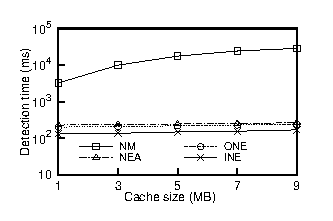
\includegraphics
   [height=3.5cm]{figure/A-size-time.eps}}
   \subfigure[{\footnotesize Beijing}]
   {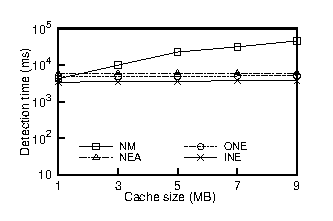
\includegraphics [height=3.5cm]{figure/A-size-time-beijing.eps}}
   \subfigure[{\footnotesize Singapore}]
   {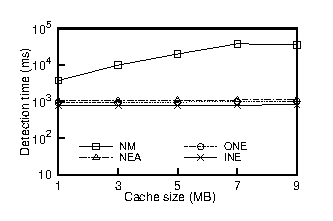
\includegraphics [height=3.5cm]{figure/singapore-detectaffect-time.eps}}
 \caption{Performance of affected path detection methods.}
 \label{fig:comparison-detecttime}
\end{figure}

%In addition, we can see the detection time is generally proportional to the size of graph.
%Aalborg has minimal time cost, Singapore has mediate time cost, and Beijing has the most time cost. The graph of Aalborg is sparse, the graph of Singapore is intermediate, and Beijing is dense. The denser a graph is, the more time it will cost because the algorithms check more paths in a dense graph to yield affected paths.

\subsection{Performance of Refreshment Strategies}
\label{ssec:overhead-strategy}

Figure~\ref{fig:comparison-hit} shows the hit-ratios of four refreshment strategies under different scales of caches.
We sum up hit ratio of 50 instances for ease of read, since the differences among strategies are tiny.
We can observe that RWC and RLB achieve the highest hit ratio. The reason is that even though RWC and RLB are based on different logics to update caches, the paths which are loaded into the cache are actually the same.
The hit ratios of RHF and RRWS are similar and a little bit worse than the former two. This result is consistent with the logics of methods, since RHF and RRWS are not fully based on large benefit values.
From the perspective of cache size, when the cache size increases, the cache will hold more paths. The cache will answer more queries, subsequently, the hit ratio increases.


\begin{figure}[htbp]
\centering
   \subfigure[{\footnotesize Aalborg}]
   {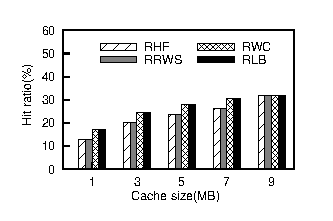
\includegraphics
   [height=3.5cm]{figure/aalborgHitVsCacheSize.eps}}
   \subfigure[{\footnotesize Beijing}]
   {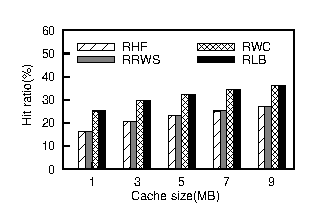
\includegraphics [height=3.5cm]{figure/beijingHitVsCacheSize.eps}}
   \subfigure[{\footnotesize Singapore}]
   {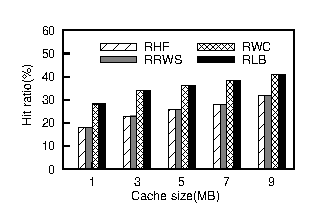
\includegraphics [height=3.5cm]{figure/singaporeHitVsCacheSize.eps}}
 \caption{Hit ratios of refreshment strategies.}
 \label{fig:comparison-hit}
\end{figure}


Next we test the refreshment time of these four replacement strategies along with various cache sizes on three data sets.
The refreshment time includes three parts: the time of detecting affected paths, the time of computing shortest paths by the server, and the time of selecting new paths into the cache. For RWC, the time of detecting affected paths is zero.
The experimental result (rf. Figure~\ref{fig:comparison-overall-time}) on each data set is the average of 50 instances.
The performance on three data sets is consistent; each method displays similar trends on three data sets.
RWC spends the most refreshment time, and the time increases as the cache size increases. It can be predicted that the disadvantage of RWC in refreshment time will amplify more if more shortest paths are queried, since RWC takes a lot of time to computing shortest paths every time the cache is emptied.
RLB, RHF, and RRWS spend similar time.
Precisely, RLB has the shortest refreshment time.
This is consistent with our analysis in Section~\ref{sec:strategies}.
 \begin{figure}[htbp]
\centering
   \subfigure[{\footnotesize Aalborg}]
   {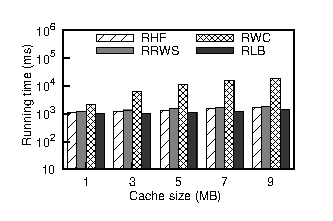
\includegraphics
   [height=3.5cm]{figure/A-size-method-time.eps}}
   \subfigure[{\footnotesize Beijing}]
   {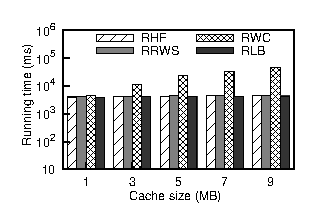
\includegraphics [height=3.5cm]{figure/A-size-method-time-beijing.eps}}
   \subfigure[{\footnotesize Singapore}]
   {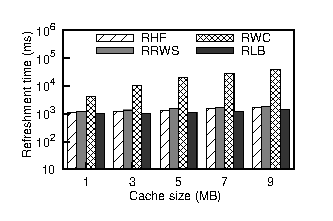
\includegraphics [height=3.5cm]{figure/SinggporeCache-size-time.eps}}
   \caption{Refreshment time of refreshment strategies.}
   \label{fig:comparison-overall-time}
\end{figure}

From the above experiments, we can see that RLB has the best running time and hit ratio. Hence, in the real applications, RLB is suggested to be used.




\section{Conclusions}
\label{sec:con}
We address the problem of refreshing cache contents in a changed network.
Changes of road conditions are commonly seen in the real world, i.e., traffic congestion or road constructions.
Shortest path caches need refreshing periodically, so that the information is accurate and valid and the cache utilization is maximized.
To the best of our knowledge, our work is the first one to discuss the cache refreshment problem when an edge changes its weight.
In order to store shortest paths and answer queries efficiently, a bitmap-based cache structure is used.
We introduce the concept of affected paths, and then exploit the properties associated with affected paths.
In the following, we develop algorithms to detect affected shortest paths resulted from road network changes.
Sequentially, four cache refreshment strategies are illustrated.

A series of experiments are conducted. The performance of cache structure and affected path detection methods are considerable.
Computational results showcase that RLB is as good as RWC in terms of hit ratio while the former has a much shorter refreshment time.
Our work has many applications, such as refreshment of shortest paths caches of map companies.
We suggest that RLB is used to refresh caches at short intervals and RWC is used at long intervals. How to trade off the use frequency of two methods is based on the real applications.

The weakness of our work, even of most works of this kind, is that we rely heavily on the information of query logs, although we introduce roulette wheel selection to avoid over fitting.
It is clearly that future queries are not a precise copy of query logs. Hence, the hit ratio is to some extent restricted by query logs.
In the future, works may focus on the following directions. The cache structure, the method to detect affected paths and the strategies to refresh caches can be studied solely and then consolidated, obtaining a strengthened cache refreshment solution. The problem of ``batch of updates'' should be considered. In this paper, we only consider the change of single edge. The story of batch changes is not a simple repetition of single change, since edges could interfere. The impact of multiple edges is combinatorial.
Currently we just consider the changes of the graph; it would be interesting to investigate the changes of query patterns. Of course, it may be possible to study directed networks in the future as in the real life one direction of a road may be closed for construction or other purposes while the other direction is still open.

\subsubsection*{Acknowledgments.}
{The work is partially supported by the National Basic Research Program of China (973 Program) (No. 2012CB316201), the National Natural Science Foundation of China (No. 61322208, 61272178, 61129002), the Doctoral Fund of Ministry of Education of China (No. 20110042110028), the Fundamental Research Funds for the Central Universities (No. N120504001, N110804002), and the Support Plan for Young Teachers of Shanghai (No. ZZSD15095).}




\section*{References}
\bibliography{refresh_cache}
\end{document}

